%!TEX root = Thesis.tex

\chapter{Parallel Hierarchical Synthesis}\label{chap:hsf} 

  To elaborate the advantages of both deterministic optimization and circuit simulation, this work tends to integrated them as a hierarchical process. The framework inherit synthesis flow in \cite{PerfMap_ISQED2011} mostly. Here the updated flow replace the original performance exploration with PGA methodology. Also, the fine-tuning simulation is improve as probabilistic perturbation simulation. Therefore, our proposed flow is shown in Figure~\ref{fig:PageFlow}, and the corresponding notations are list in Table~\ref{table:notation}.

  


  \section{Device Fitting}\label{sec:devFit}
    
    At the beginning of synthesis framework, we have an abstraction from device model to circuit-level variables. Given the required devices of the target circuit design, the foundry device models provide such device characteristics with SPICE modeling. A set of analytical design equations are capable to map device-level variables into circuit-level design variables by modeling techniques such as symbolic analysis or curve fitting like~\cite{PWL_Convex_GP,Eeckelaert_DATE2003,Daems_DAC2002}. Two steps of technique accomplish the abstraction for design variables. 

    First of all, it is necessary to discover feasible variable values for each attendant device. In other words, all design variable values which cause device failed should be exclusive at this stage. By SPICE simulator, a matrix of accessible device level variable value are generated. However, since this step is collecting the feasible range of each device level parameters, the table is collected in one-time. 
    
    \begin{figure}[t]
      \centering
      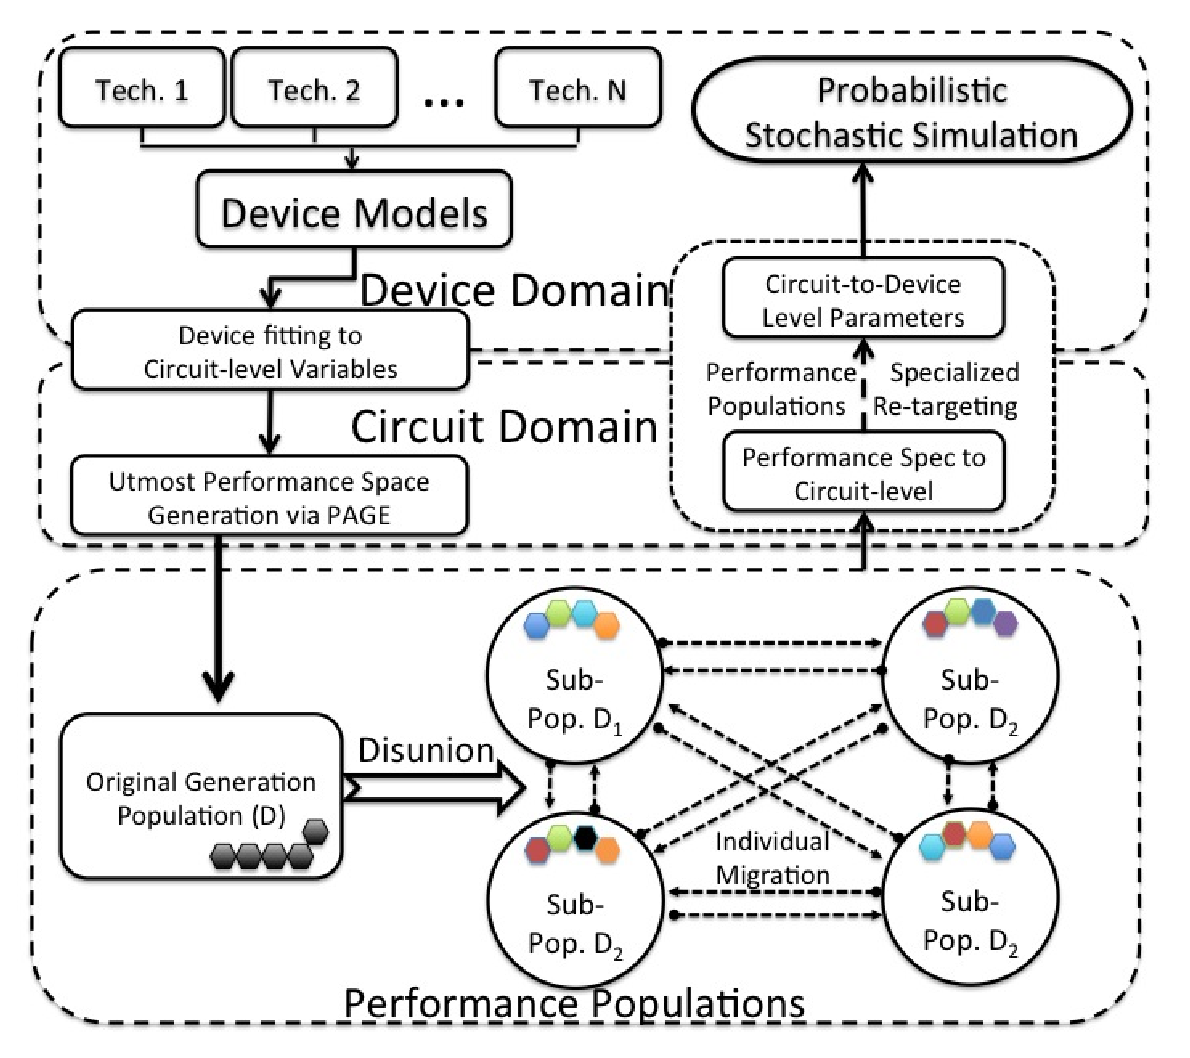
\includegraphics[width=\textwidth]{Fig/PageFlow.eps}
      \caption{Hierarchical performance exploration flow with PGA} 
      \label{fig:PageFlow}
    \end{figure}

    Secondly, such matrix of device-level variables are further mapped into circuit-level variables by curve fitting. An vivid example for design variable mapping is shown in Figure~\ref{fig:DeviceFit}. Given a set of device-level variables $V^D= \{{v^D}_i| 1 \leq i \leq |V^D|\}$ , each $v^D_i$ has the same step number $S_{V^D}$ in each range. That is, while $v_i^D$ has maximum value $V^D_{MAX}$ and minimum value $V^D_{min}$, there should be $S_{V^D}$ values among then. Therefore, a set of feasible device-level variables are constructed in a matrix $T_{|V^D|\times S_{V^D}}$, where $T_{|V^D| \times S_{V^D}} = \{ t_{i,j}| 1 \leq i \leq |V^D|, 1 \leq j \leq S_{V^D} \}$. Meanwhile, a set of circuit-level variables $V^C = \{{v^C}_j| 1 \leq j \leq |V^C|\}$ should be extracted for performance exploration. As Eq.(\ref{eq:devToCir}),all training pairs of the extracted circuit-level variables from previous transformation and device-level variables are then formulated as least-square error problem in analytical posynomial form design equations to acquire fitting parameters.

    {\footnotesize
    \begin{align}\label{eq:devToCir}
      \begin{array}[t]{rl}
        Variables: & \begin{array}[t]{rl}
                      T_{|V^D| \times S_{V^D}}  & = \{t_{i,j}| 1 \leq i \leq |V^D|,\; 1 \leq j \leq S_{V^D}\}   \\
                      V^C   &= \{v_j^C, 1\leq j \leq |V^C| \}   \\
                      v_j^C &= \{f_j^{(C_f)}(T_{|V^D| \times S_{V^D}})|1 \leq j \leq |V^C|\}  \\
                    \end{array} \\
         minimize & \| \sum{ v_j^C - f_j^{(C_f)}(T_{|V^D| \times S_{V^D}})}\|^2   \\
       subject\; to & C_f\in \left [{C_f}_{min}, {C_f}_{MAX} \right] 
      \end{array} 
    \end{align}}
    
    
    where
    \begin{itemize}
      \item $C_f$ is the fitting parameters of $f_j$ 
      \item $\left [{C_f}_{min},{C_f}_{MAX}\right]$ is the range constraints of the fitting parameters in $f_j, 1 \leq j \leq |V^C|$.
    \end{itemize}

    Since parasitics are non-ignorable, the parasitic effects of devices should also be extracted for the following steps in order to exploit the trade-off between each aspect of circuit design variables and performance metrics.~\cite{Template_Based_Parasitic_Aware_Layout}. The problem formulation is similar to Eq.(\ref{eq:devToCir}) in Eq.(\ref{eq:paraExt}):
  
    \vspace{0.3cm}
    {\footnotesize
      \begin{align}\label{eq:paraExt}
        \begin{array}[t]{rl}
        Variables:  & \begin{array}[t]{ll}
                        T_{|V^D| \times S_{V^D}} &= \{t_{i,j}| 1 \leq i \leq |V^D|,\; 1 \leq j \leq S_{V^D}\}   \\
                        V^P     & = \{v^p_l|1 \leq l \leq |V^P|\} \\
                        v^p_l   & = \{Q_l^{(C_p)}(T_{|V^D| \times S_{V^D}})| 1 \leq l \leq |V^P| \}
                      \end{array} \\
        minimize    &  \| \sum{v^p_l-Q_l^{(C_v^p)}(T_{|V^D| \times S_{V^D}})}\|^2  \\
        subject to  &  C_v^p \in \left [ {C_v^p}_{min}, {C_v^p}_{MAX}\right] 
        \end{array} 
      \end{align}
    }
    where

    \begin{itemize}\setlength{\itemsep}{2pt}
      \item $v^p_l$ is the mapping equations from $T_{|V^D|\times S_{V^D}}$ to $V^P$, 
      \item $C_p$ is the fitting parameters of $Q_l$,
      \item $\left [ {C_{v^p}}_{min}, {C_{v^p}}_{MAX}\right]$ is the range constraints of the fitting parameters in $Q_l$.
    \end{itemize}

  
    \begin{figure}[t]
      \centering
      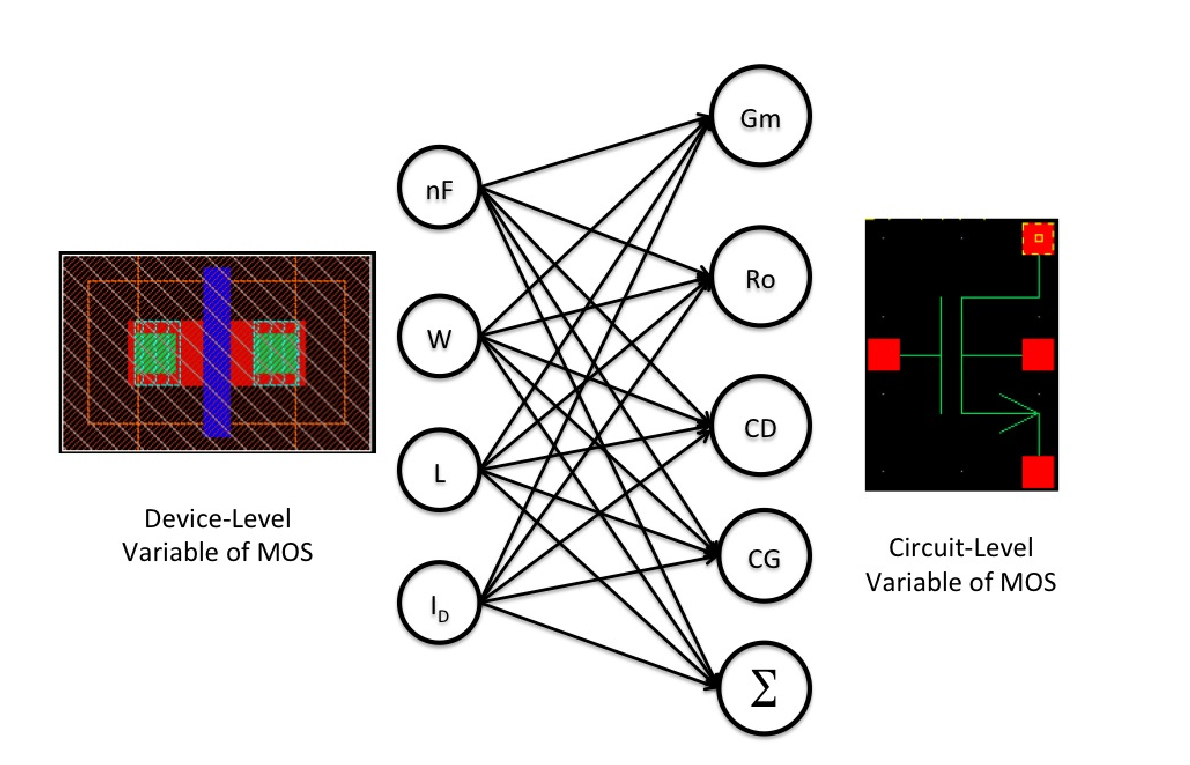
\includegraphics[width=\textwidth]{Fig/DeviceFit.eps}
      \caption{Mapping device-level variables of one NMOS(number of fingers, device channel width/length and current) to circuit-level variables ($G_m$, $R_o$, $C_D$, $C_G$ and $\Sigma$) } 
      \label{fig:DeviceFit}
    \end{figure}

  
  %!TEX root = Thesis.tex

  \section{Performance Space Exploration with Parallel Genetic Algorithm}\label{sec:pga}
    
    \begin{figure}[t]
      \centering
      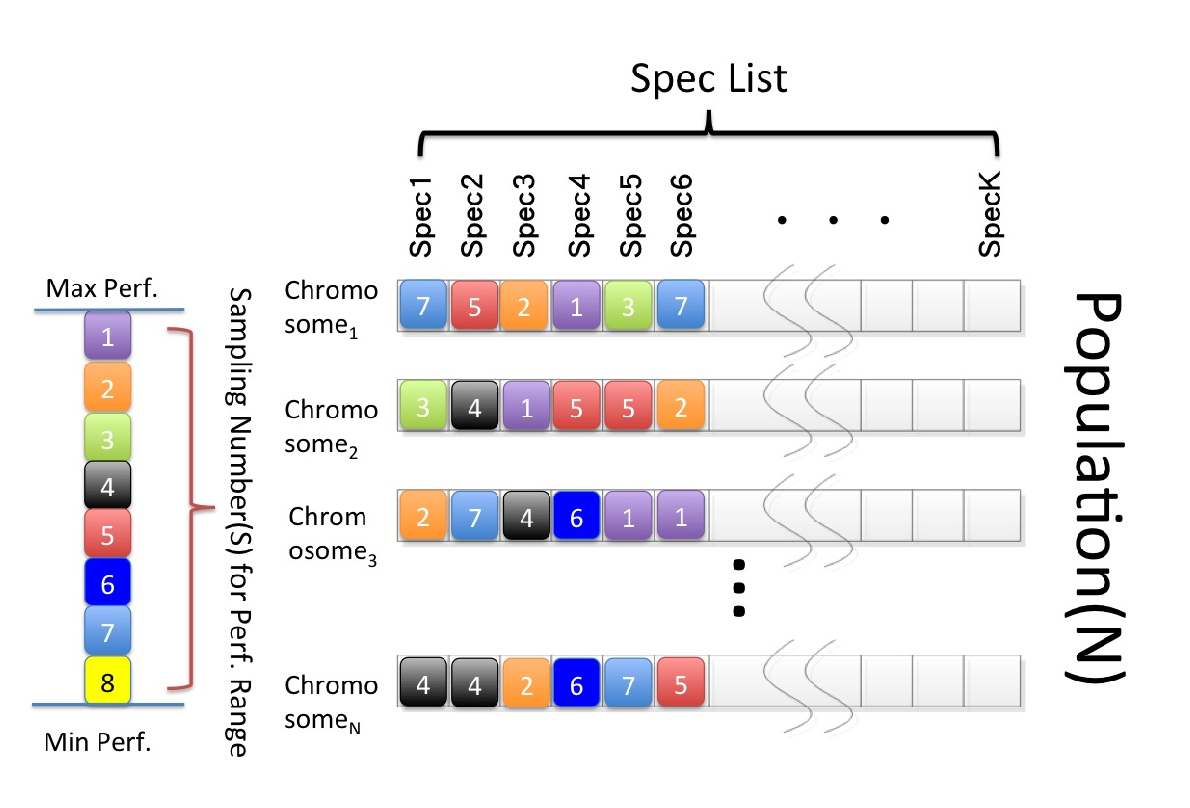
\includegraphics[width=\textwidth]{Fig/Gene.eps}
      \caption{Demonstration of genetic representation for performance metrics.} 
      \label{fig:Gene}
    \end{figure}

    To traverse the space of required circuit performance, we propose an efficient exploration process to investigate the feasible performance metrics of such analog design. Once the set of circuit-level design variables $V^C$ are prepared, these variables can be adopted as parameters into circuit design equations. A set of design equations along with circuit-level parameters, parasitic effects and fitting parameters are constrained with performance requirement. Note that the parasitic effects of the devices are included so as to explore the trade-off between each aspect of performance metrics and circuit-level design variables. To figure out the design equation set with performance constraints is feasible or not, we apply convex optimization. Since the circuit design equations are formulated as geometric programming by posynomial forms, the optimization to find feasible solution with performance constraints is convex. Moreover, to extend the problem with different performance specifications, that each combination of performance constraints can be checked is feasible or not. A set of specification are swept as the constraints for an optimization performance to get performance metrics.
 
    An optimization problem in Eq.(\ref{eq:DesignEq}) describes a unit performance optimization step.

    \begin{align}\label{eq:DesignEq}
      \begin{array}{ll}
      Variables:  & \begin{array}[t]{ll}
                        V^C & = \{{v_k}^C | 1 \leq k \leq |V^C|\} \\
                        V^P   & = \{ v^p_k | 1 \leq k \leq |V^P| \}\\
                        F   & = \{ f_k | 1 \leq k \leq |F| \}\\
                        R   & = \{ r_k | 1 \leq k \leq |R| \} 
                    \end{array}                 \\
        minimize  &   f_{OBJ}( {v_i}^C,v^p_k,f_k)         \\
      subject\ to & \begin{array}[t]{l}
                    r_1 = Perf_1(V^C,V^P,F) \geq z_1\\
                    r_2 = Perf_2(V^C,V^P,F) \geq z_2\\
                    \vdots \\
                    r_k = Perf_k(V^C,P,F) \geq z_k
                \end{array}             
      \end{array}
    \end{align}
    where
    \begin{itemize}
      \item  $V^C$ is circuit level variables extracted from device-level variables.
      \item  $V^P$ is a set of parasitics which is non-ignorable for circuit modeling.
      \item  F demonstrates fitting parameters to fit from circuit-level parameters to performance space.
      \item  R represents the corresponding performance result set which obtain by optimization. 
      \item  $Z = \{z_k| 1 \leq k \leq |Z|\}$ is a set of performance required value. In other words, each $z_k$ represents a value of performance constraint, eg. $z_k \geq 40 \to Av \geq  40dB$
    \end{itemize}
    \vspace{0.3cm}

  
    In every optimization process, one performance metric results in a set of performance metric ($r_1 ,\ldots, r_k$) corresponding to the given specification of performance($z_1,\ldots,z_k$). Therefore, according to the same design equation for optimization, it is an one to one mapping relationship from spec to result of performance and the corresponding circuit-level design variables. 

    To extend the optimization range. Each $z_k$ can be varied with a range of value, that is, we define a maximum value of $z_{kMAX}$ and one minimum value of $z_{kmin}$ with several step value between them. Therefore, we can investigate the performance limitation for $z_k$ by implementing optimization on a series of $z_k$, $z_k=\{z_{ki}| 1 \leq i \leq |z_k|, z_{kMAX} \leq z_{ki} \leq z_{kmin} \}$. Obviously, a set of different performance types with a range of such values are similar to chromosome concept in heredity. As we can see in Fig.~\ref{fig:Gene}, if every chromosome carries different value of every performance metric $z_k$. An evolutionary computing with genetic algorithm for traversing solution space can be employed for traversing optimized multi-objective problem. As mentioned in Section~\ref{sec:PGAIntro}, we further utilize the {\it Parallel Genetic Algorithm} to develop with. The detail implementation is as follows:

    


    \subsection{PGA Overview}

      The methodology to exercise PGA fusion with performance exploration is shown in Algorithm~\ref{alg:PGA}. PGA traverses the performance space by evolution. According to \cite{SurveyDistPGA1997}, our approach picks the coarse-grained fashion PGA. In traditional genetic algorithm, one major population has numbers of individual chromosomes for evolution. In coarse-grained genetic algorithm, the major population is separated into numbers of sub-populations with the same size of individual. Since each sub-population contains large number of individuals, it is time-consuming to exercise fine-grained structure. Therefore, the coarse-grained structure is much efficient at this situation. 


      \begin{figure}[t]
        \centering
        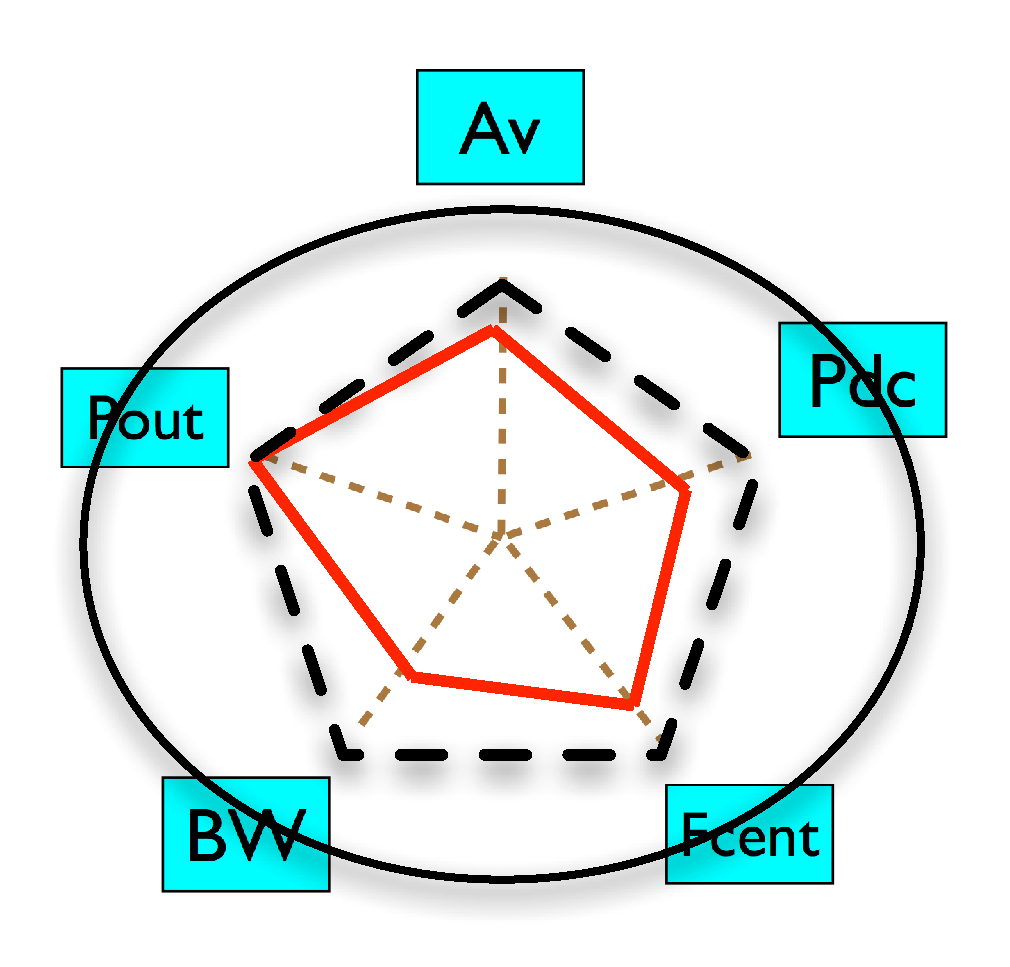
\includegraphics[width=\textwidth]{Fig/MultiSpec.eps}
        \caption{Illustration of performance characteristic (e.g., Av, Pdc, Pout, BW, Fcent, etc.) for each circuit.} 
        \label{fig:MultiSpec}
      \end{figure}


      \newcommand{\PGA}{\ensuremath{\mbox{\sc PGA}}}
      \algloopdefx{RETURN}[1][]{\textbf{return} #1}
      \algblockdefx{FORALLP}{ENDFAP}[1]%
      {\textbf{for all }#1 \textbf{do in parallel}}%
      {\textbf{end for}}
      \begin{algorithm}[t]  
        \caption{$\PGA(Z_{K\times S},N_P,S,k,T,C,M_P)$}\label{alg:PGA}                       
        \begin{scriptsize}
          \begin{algorithmic}[1]
            \REQUIRE 
              \begin{tabular}{l}
              $Z_{K\times S}$: Performance Space Matrix. \\
              $N_P$: Number of Individuals in major population.\\
              %$N_S$: Number of sub-populations.\\
              S: Sampling number for each performance spec $z_k$\\
              K: Number of Performance spec type\\ 
              T: Technology type. \\
              C: Circuit type.\\
              $M_P$: Migration rate.
                \end{tabular}
            \ENSURE 
              \begin{tabular}{l}
                $R_{K \times S}$ : The result performance space\\
                    $P$ : The population of performance specs after PGA
                  \end{tabular}
              \FOR {$i = 1 \to N_P$}
                \FOR {$j = 1 \to k$}
                  \STATE $G_i \gets RandGetSpec(Z_{j\times S})$ \COMMENT{Randomly generate spec value from Z}   
                \ENDFOR
                \STATE $P \gets G_i$
              \ENDFOR
              \FOR {$i = 1 \to k$}
                \STATE $P_i \gets Partition(P,i)$
              \ENDFOR
              \WHILE {Convergence criterion satisfied}          
                \FORALLP {$i = 1 \to k$} 
                  \STATE $R_i \gets Evaluate(P_i,T,C)$
                  \STATE ${Pool}_i \gets Reproduction(P_i,Fitness(T,C,i,R_i))$
                  \STATE $P_i \gets Crossover(P_i,{Pool}_i)$
                  \STATE $P_i \gets Mutation(P_i)$
                \ENDFAP   
                \FOR {$i = 1 \to k$} 
                  \STATE $Migration(P_i,exclusive(P,P_i),M_P)$
                \ENDFOR 
              \ENDWHILE
              \STATE $P \gets Merge(P_1,P_2, \ldots, P_{k})$
              \RETURN $P, R_{K \times S}$  
          \end{algorithmic}
          \end{scriptsize} 
      \end{algorithm}

      As for analog performance optimization, which is a multi-objective problem with a Pareto-front as illustrated in Fig.~\ref{fig:MultiSpec}. To find the Pareto-front, each performance target optima should be traverse as well. Therefore, we further use heterogeneous coarse-grained structure for evolution. In other words, every sub-population deals with different objective that performs optima. For example, one sub-population implement performance exploration to evolve population with better voltage gain($A_v$). Therefore, we pick the fitness function which emphasizes on such performance item($A_V$). Moreover, each sub-population has its own fitness function and evolve independently. Additionally, the diversity for the overall population also can be maintain by migration strategy in the end of the performance exploration stage.

    \subsection{Chromosome Encoding}

      Before PGA process, the fundamental chromosome encoding should be defined. For one performance target $z_k$, given performance upper and lower bound, $\{\left [z_{kmin},z_{kMAX} \right]$. There exist a set of discrete $z_{k,s}$ among this boundary, where 
      \begin{defi}\label{def:Z}
        $\forall z_k, \exists z_{k,s} \to z_{k,S} = \{z_{kmin} \leq z_{k,s} \leq z_{kMAX}\}$. As Algorithm~\ref{alg:PGA} mentioned in $Input:$, S denotes the sampling number for each $z_k$. Therefore, $z_{k,s} = \{z_{kmin} + ({z_{kMAX}-z_{kmin}})\times s/S | 1 \leq s \leq S\}$
      \end{defi}

      \begin{align}\label{eq:PerfMatrix}
        \begin{array}{rl}
          Z_{K \times S} & = 
              \left[\begin{array}{cccc}
               z_{11} & z_{12} & \dots  & z_{1S} \\
               z_{21} & z_{22} & \dots  & z_{2S} \\
               \vdots & \vdots & \vdots & \vdots  \\
               z_{K1} & \dots  & \dots  & z_{KS} 
            \end{array}\right]
        \end{array}
      \end{align}
   
      where
      \begin{itemize}
        \item K: the number of performance specification types. (eg: Av, BW,...,etc.)
        \item $\left[Z_{min},Z_{MAX}\right]_{k}$, $k = 1, \ldots, K$ is the $k_{th}$ type specification range of the performance space.
        \item S is the sampling number for each $Z_S$ between ${Z_k}_{min}$ and ${Z_k}_{MAX}$.
        \item  $\forall z_{ki} \in Z_{K \times S}$, if $i= 1$, $z_{ki}= {Z_S}_{min}$ and if $i = S$, $ z_{ki}={Z_S}_{MAX}$
      \end{itemize}

      By Definition~\ref{def:Z}, every $z_{k,s}$ for $z_k$ are selected as constraints for an optimization problem which represents the circuit design equation. Here we expand the performance space as an $S \times N$ matrix in Eq.(\ref{eq:PerfMatrix}). Moreover, each performance spec from constraints is is encoded as chromosome G from maximal to minimal in a set of $G = \{g_k| 1 \leq k \leq K\}$. For example, $g_i \in G$ randomly obtains value of the $k^{th}$ spec from $z_{k,1}$ to $z_{k,S}$.

    \subsection{Initialization}
      As algorithm~\ref{alg:PGA} described in $Input$, a set of performance space matrix $Z_{K \times S}$ is given. First of all, a major population is constructed according to $Z_{K \times S}$. Algorithm~\ref{alg:PGA} Line 1 to Line 6 illustrate the process to assign performance specs as chromosome for each individual of the major population iteratively. For the reason that we want to achieve multi-objective optimization, k sub-populations are generated and evolved independently. Therefore, a major population $P$ is generated. According to the size of sub-population $k$, master processor allocates individuals to each slave processor uniformly as sub-population $P_1 \ldots P_{k}$. 
  
    \subsection{Evolution}

      An evolution is executed between Algorithm~\ref{alg:PGA} Line 10 and Line 20. Because the $Evaluate$, $Reproduction$, $Crossover$ and $Mutation$ parts are independent, the parallel parts can be performed from algorithm~\ref{alg:PGA} Line 11 to Line 16. Hence, in each sub-population, each location of gene in one individual is fed into $Evaluate(P,T,C)$ as target constraints for performance to the design equation(shown in Eq.(\ref{eq:DesignEq})) and a corresponding result $R_i$ is obtained. However, if one combination of performance metrics produces the solution space which is not convex, such individual would be failed by $Evaluate$. Then, a random generated individual replaces and redoes $Evaluate$ again until each chromosome $G$ has obtained its corresponding result $R = \{r_k| 1 \leq k \leq|R| \}$. 
      
      Fig.~\ref{fig:PGAFlow} shows the flow of the parallel genetic evolution from random performance space matrix($Z_{K\times S}$) to convergence. Each sub-population experiences a evolution with $Evaluate$, $Reproduction$, $Crossover$ and $Mutation$. Between algorithm~\ref{alg:PGA} Line 12 to Line 15, parallel genetic algorithm utilizes a fitness function to determine the suitability for each $G_i$. In our algorithm, we use the $Heterogeneous\ Island$ architecture \cite{SurveyCGPGA1994}. According to our requirement, we tend to specialize the particular spec, such as voltage gain($A_v$). A set for fitness function is given, $Fitness = \{{fitness}_i| 1 \leq i \leq k\}$ as kind of objective function to determine how important each individual is with the $Evaluate$ result. Each sub-population $P_i$ applies one particular fitness function which is related to the required performance result $R_k$ of $Evaluate$ value. Therefore, the fitness function determines the qualified individuals to be preserved to the crossover pool in a weighted ratio, and the others should be extinct. In $Crossover$ of algorithm~\ref{alg:PGA} Line 14, the $Crossover$ step selects each two genes $G_i$ and $G_j$ ,where $\{G_i,G_j \in Pool; 1 < i<j<N\} $ for copulation. Since each individual has $K$ types of spec, these two individuals exchange {\bf c} specs and reserve {\bf $K-c$} specs with each other. In the end of parallel sub-level evolution, the {\it Mutation} step picks up one individual with mutation rate and then replaces one gene value by one slot of $Z_K$. 
    
      \begin{figure}[t]
        \centering
        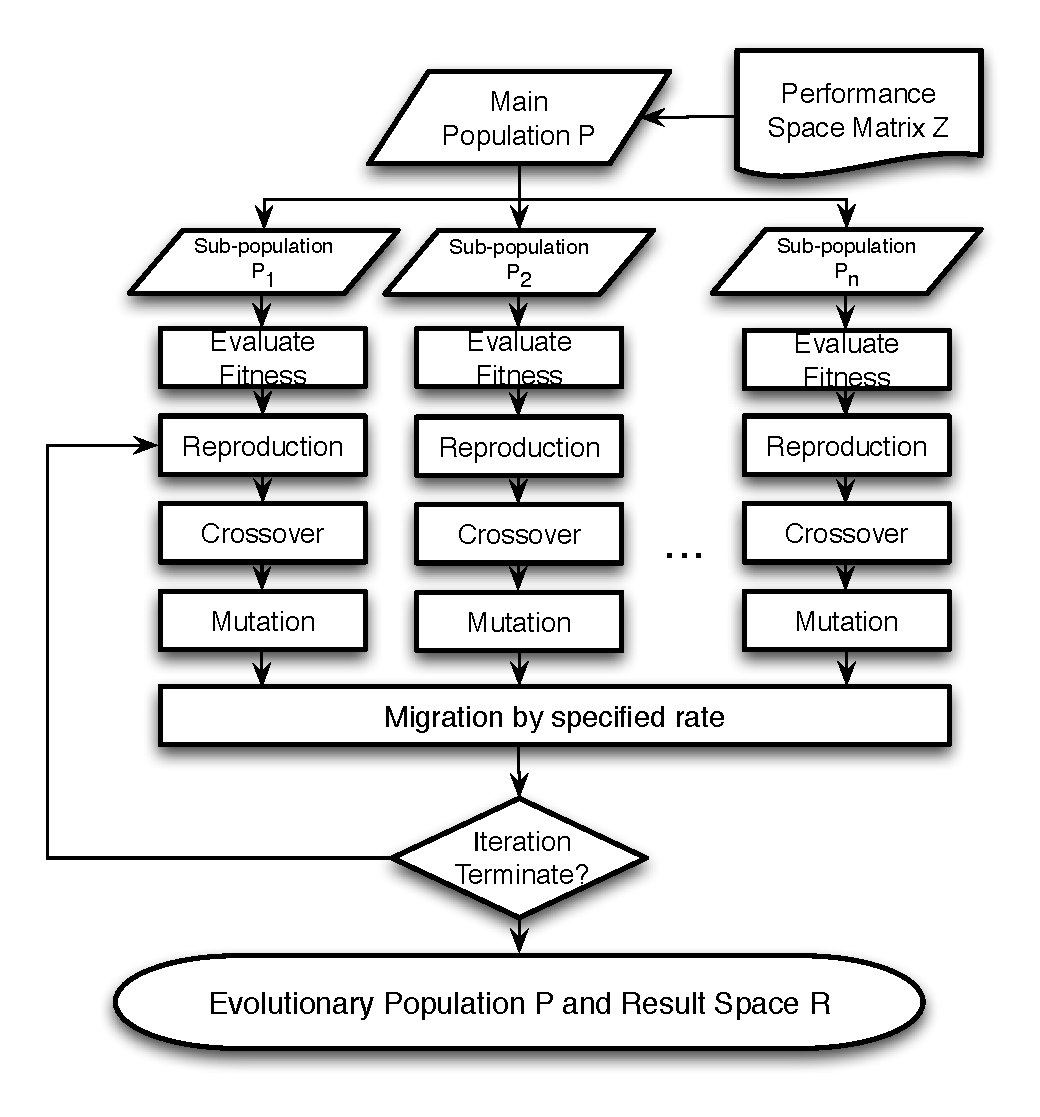
\includegraphics[width=\textwidth]{Fig/PAGEflowchart.eps}
        \caption{Coarse-grained parallel genetic approach from major population P to partitioned population $P_i$ for parallel evolution. The migration step benefits each sub-population on diversity every iteration.} 
        \label{fig:PGAFlow}
      \end{figure}

    \subsection{Migration}  

      \newcommand{\Migration}{\ensuremath{\mbox{\sc Migration}}}
      \algloopdefx{RETURN}[1][]{\textbf{return} #1}
      \algblockdefx{FORALLP}{ENDFAP}[1]%
      {\textbf{for all }#1 \textbf{do in parallel}}%
      {\textbf{end for}}
      \begin{algorithm}[t]  
        \caption{$\Migration(P_i,exclusive(P,Pi),M_P)$}\label{alg:Migration}                       
        \begin{scriptsize}
          \begin{algorithmic}[1]
            \REQUIRE 
              \begin{tabular}{l}
              $P_i$: The population which want to migration, where $i = 1... k$\\
              $exclusive(P,P_i)$: Return a population set except $P_i$ .\\
              %$N_S$: Number of sub-populations.\\
              $M_P$: Migration rate.
                \end{tabular}
            
              \FOR {$j = 1 \to k$}
                  \IF{$j \neq i$}
                    \STATE $R_P \gets rand(0,1)$
            \IF{$R_P \leq M_P$}
                      \STATE  $I_S=bestIndividual(P_i,fitness(T,C,j,R_i))$
              \STATE  $I_R=worstIndividual(P_j,fitness(T,C,j,R_j))$
              \STATE  $replaceIndividual(P_i,P_j,I_S,I_R)$
            \ENDIF
          \ENDIF
                \ENDFOR
             
              \STATE $P \gets Merge(P_1,P_2, \ldots, P_{k})$
              
          \end{algorithmic}
          \end{scriptsize} 
      \end{algorithm}

      In the end of each independent evolution, we perform $Mutation$ with a given mutation rate for sub-population $P_i$ from 1 to $K$. Later, every sub-population is updated. Then, $Migration$ is summarized as shown in Algorithm~\ref{alg:Migration} aims to exchange individuals in the population network shown in the bottom of Fig.~\ref{fig:PGAFlow}. Therefore, each $P_i$ should operate $Migration$ with the others. From algorithm~\ref{alg:Migration} Line 5 to Line 7, each $Migration$ between $P_i$ and $P_j$, $P_i$ exchanges its best individual with respect to ${fitness}_j$, and $P_j$ replaces its worst individual with respect to own ${fitness}_j$ with migration rate $M_P$ in algorithm~\ref{alg:Migration} Line 4. Different sub-population owns its fitness function and uses the particular migration strategy can close to natural evolution. An example of a migration operation between two sub-populations is shown in Fig.~\ref{fig:Migration}. After the $Migration$ is executed, the composition of each $P_i$ is updated with higher diversity. 
    
    \subsubsection{Merge}
      After all, while the termination condition meets, all the sub-populations are generated. These sub-populations not only have good solution with respect to all spec, but also enhance diversity. All individuals in each sub-population merge to a main population one after another. After merge, main population has all the individuals generated from evolution. 
  
  
      \begin{figure}[t]
        \centering
        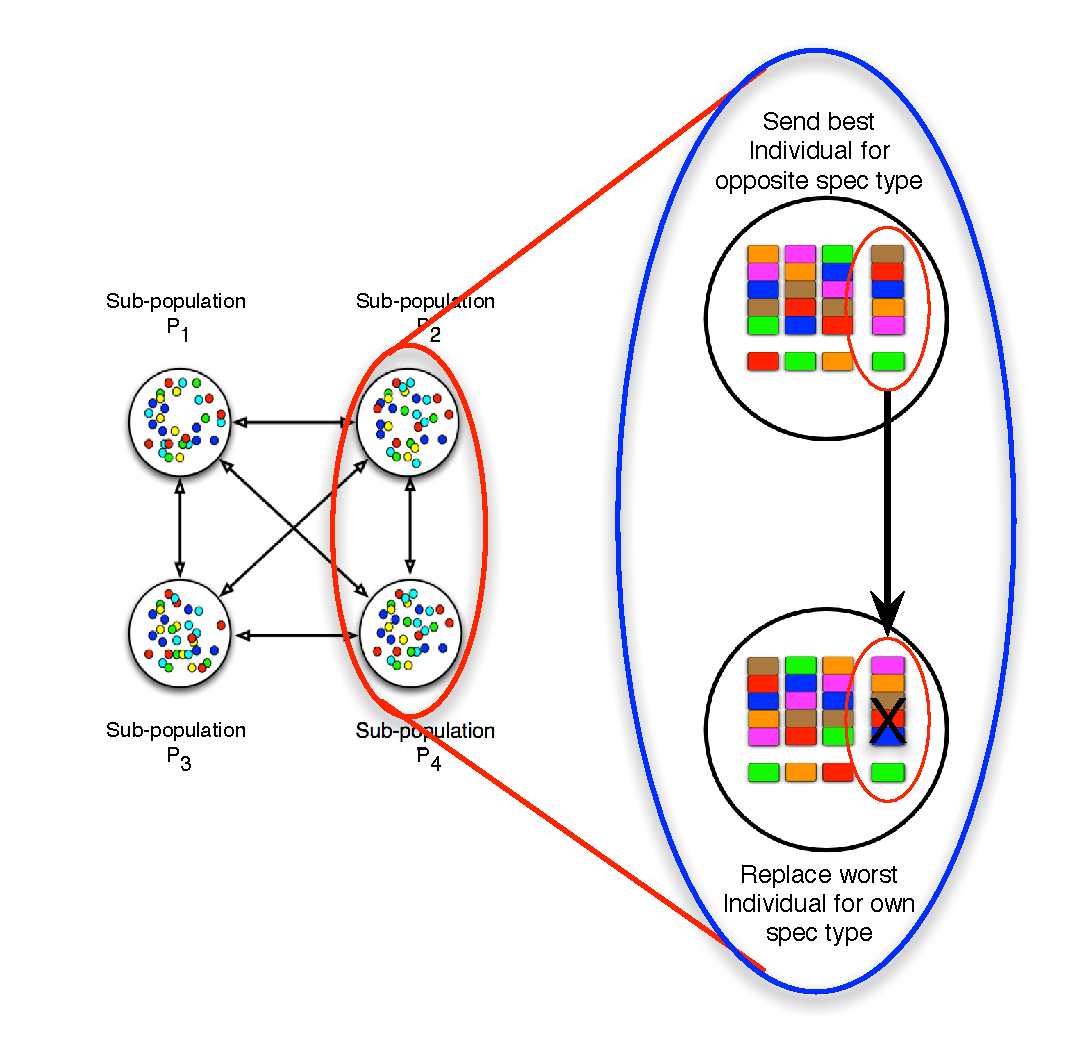
\includegraphics[width=\textwidth]{Fig/PAGEMigration.eps}
        \caption{When sub-population $P_2$ and sub-population $P_4$ perform migration operation with migration rate $M_P$, $P_2$ sends its best individual with respect to spec type $P_4$, and the receiving sub-population $P_4$ replaces its worst individual with respect to its own spec type $P_4$.} 
        \label{fig:Migration}
      \end{figure}

    To consider the complexity of PGA, it is considerable to check the dimension of $Z_{K\times S}$. According to line 12 in Algorithm~\ref{alg:PGA}, $Evaluate(P_i,T,C)$ is the most critical. Each $Evaluate$ for $P_i$ need to resolve $\frac{N_P}{N_S}$ convex optimization problems in serial, which is $O(\frac{N_P}{N_S})$. Comparing to the exhaustive approach, the complexity is restricted to $K$ and $S$. That is, we need to traverse every combination from specification space in $Z_{K\times S}$ for $O(S^K)$ complexity. For example, if a circuit require two performance specs ($A_v$ and $BW$) with 4 sampling steps ($A_v = \{5,10,15,20\}$, $BW = \{3MHz,5MHz,8MHz,10MHz\}$). Therefore, the overall combination of specs need to be checked is $4^2=16$. Obviously, we can observe the gap with more specs($K\uparrow$) and greater precision in sampling($S\uparrow$). To sum up, a genetic-based approach can reduce the complexity by controlling population number and a parallel enhancement further reduce the timing complexity vi parallel number. However, the accuracy is also sacrificed as trade-off.





  \section{Design Re-targeting}\label{sec:reTarg}
    
    After generating specialized populations by PGA evolution, it comes to a reverse interpolation from a series of performance specifications through circuit-level design variables to device-level design variables. Hence, K groups of optimal-potential performance spaces of the circuit under chosen technology are traversed. Since a set of performance metrics directly represents the limitation of specifications, such group of optimal performance specification is locked from optimal performance. Ideally, the optimization engine should be capable of directly finding the geometry-biasing-level design variables. 

    Next, we want to find the optimal candidates of device-level design variables. From previous stage, the circuit-level design variables are obtained. Here the distribution of the device-level design variables are also obtained through this design re-targeting stage. As Eq.(\ref{eq:SingleReTarg}) illustrated, since each device has its particular device variables, all of them are considered for optimization. $M$ stands for a set of attendant devices in the circuit. Generally, each device has different number of variables. Therefore, $V^D_{m_k}$ represents the variable set of single $m_j$. Referring to Section~\ref{sec:pga}, Performance results $R_{S \times K}$ are obtained along with the same number($N_P$) of $V^C$ and $V^P$. Each $v^C$ and $v^P$ will re-target to a set of device-level parameter values via $f_{RE}(v^C, v^P)$ transformation. Eq.(\ref{eq:SingleReTarg}) shows a single transformation from each $v^C$ and $v^P$ to a set of device-level parameters $V^D_M$,

    \begin{align}{\label{eq:SingleReTarg}}
      \begin{array}[t]{rl}
        Variables & \begin{array}[t]{rl}
                      M         &= \{ m_j| 1 \leq j \leq |M|\} \\
                      V^D_M     &= \{ v^D_{m_j} | 1 \leq j \leq |M|\} \\
                      v^D_{m_j} &= \{v^D_{m_{j,k}}| 1 \leq k \leq |v^D_{m_j}|\}\\
                      v^C       &= f^{(C_f)}(V^D_M)\\
                      v^P       &= Q^{(C_Q)}(V^D_M)\\
                    \end{array} \\
         minimize & Q(V^D_M \to V^P)  \\
       subject\; to & V^D_M\in \left [{V^D_M}_{min}, {V^D_M}_{MAX} \right] 
      \end{array} 
    \end{align}

    \begin{figure}[t]
      \centering
      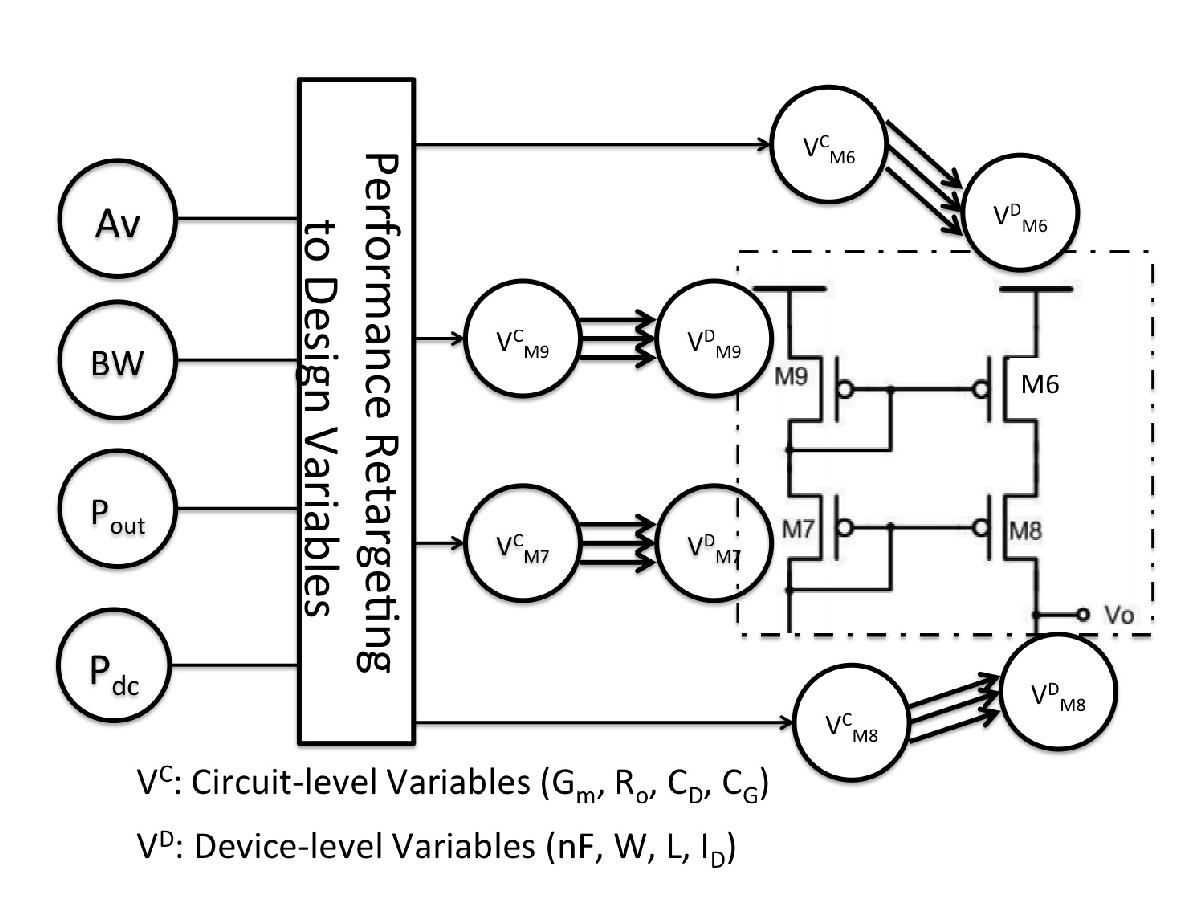
\includegraphics[width=\textwidth]{Fig/Retarg.eps}
      \caption{Given merged populations of performance specs, a reversed process is to retrieve the corresponding design variables of each device (PMOS) in the circuit for optimal sizing values.} 
      \label{fig:Retarg}
    \end{figure}
    
    In Eq.(\ref{eq:SingleReTarg}), $Q$ is a cost function that involves the parasitic effects of the device, such as a product of area, parasitic cap/resistance, or self-resonance frequency, etc. For all, Every individual $V^C$ and $V^P$ need to be transfer to device-level parameters as distributions. In Eq.(\ref{eq:FullReTarg}), $\Psi$ collects $N_P$ set of device variables for required circuit.

    \begin{align}{\label{eq:FullReTarg}}
      \begin{array}{l}
        V^C = \{v^C_i| 1 \leq i \leq N_P\}\\
        V^P = \{v^P_i| 1 \leq i \leq N_P\}\\
        \Psi =  \{V^D_{M_{i,j,k}}| 1\leq i \leq N_P, 1 \leq k \leq |M|, 1 \leq j \leq |v^D_{m_k}|\} 
      \end{array}
    \end{align}

    Also, as shown in Figure~\ref{fig:Retarg}, multiple solutions as distributions are generated from {\it Performance Space Exploration} in Section~\ref{sec:pga}, and it stands for a set of potential parameters for devices in required circuit. However, $\Psi$ not only narrows down the solution space for circuit simulation, but provides good prediction for optimal performance which will be validated via probabilistic simulation in Section~\ref{sec:pss} efficiently. 

  %!TEX root = Thesis.tex
                                            
\section{Effective Probabilistic Fine Tuning}\label{sec:pss}


  The final refinement performs a full-circuit stochastic simulation. Although we obtain a set of potential design variables from Section~\ref{sec:reTarg}, these do not represent the optimal solution. The final refinement performs simulation to prevent the solution from any non-ideal effects via higher-level abstraction. After {\it Design Re-targeting}, a set of overall device level variable values $\Psi $ are collected. $N_{V^D}$ collects the number of all device variables type. Since these design variables are selected by performance exploration via transformation, each population of performance metrics directly projects to a set of variable distribution. Basically, $\Psi$ provides the variable space for perturbation. By swapping among device-level parameters, the cost of full-circuit simulation is reduced. By employing global optimization algorithm, such as random walk or simulated annealing, the entire circuit is re-constructed and fed into circuit simulator using real models and parameters from the foundry.

  \begin{figure}[t]
      \centering
      \begin{subfigure}[t]{0.4\textwidth}
        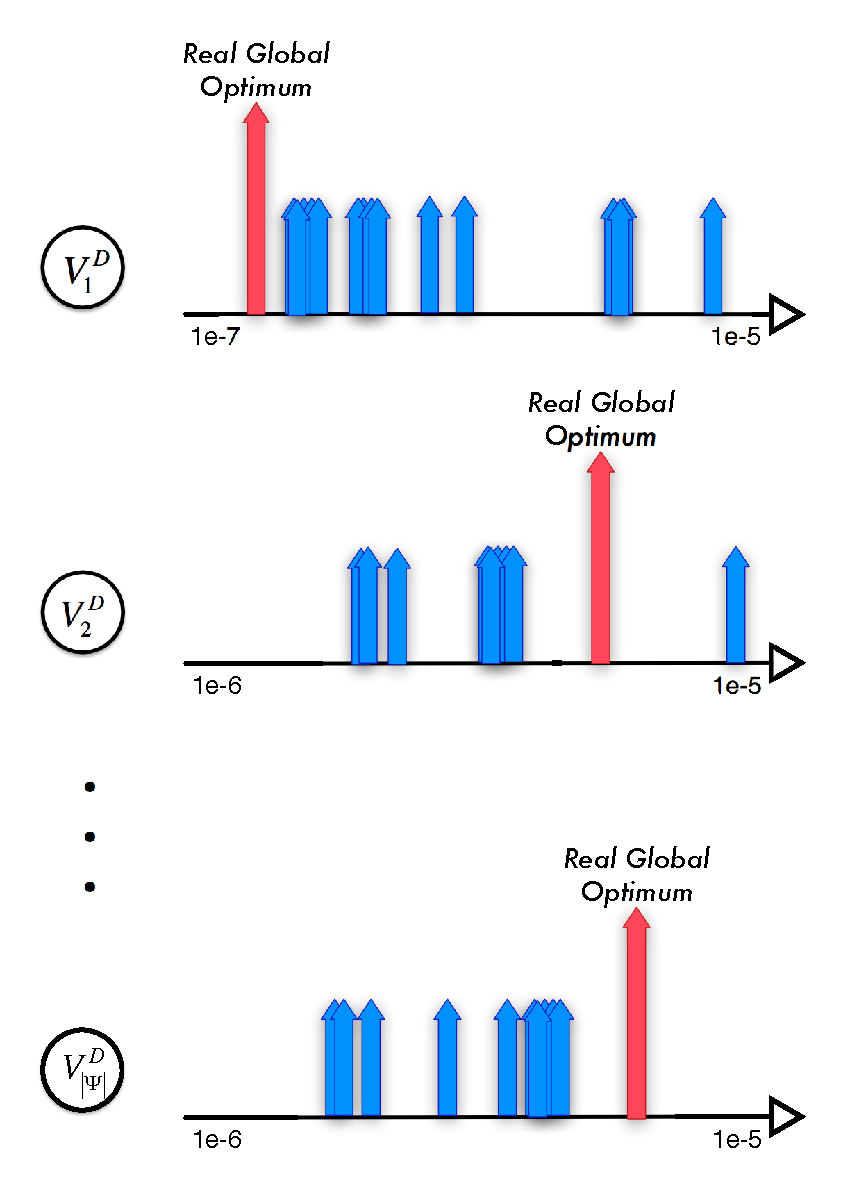
\includegraphics[width=\textwidth]{Fig/popSampling.eps}
      \end{subfigure}
      \begin{subfigure}[t]{0.4\textwidth}
        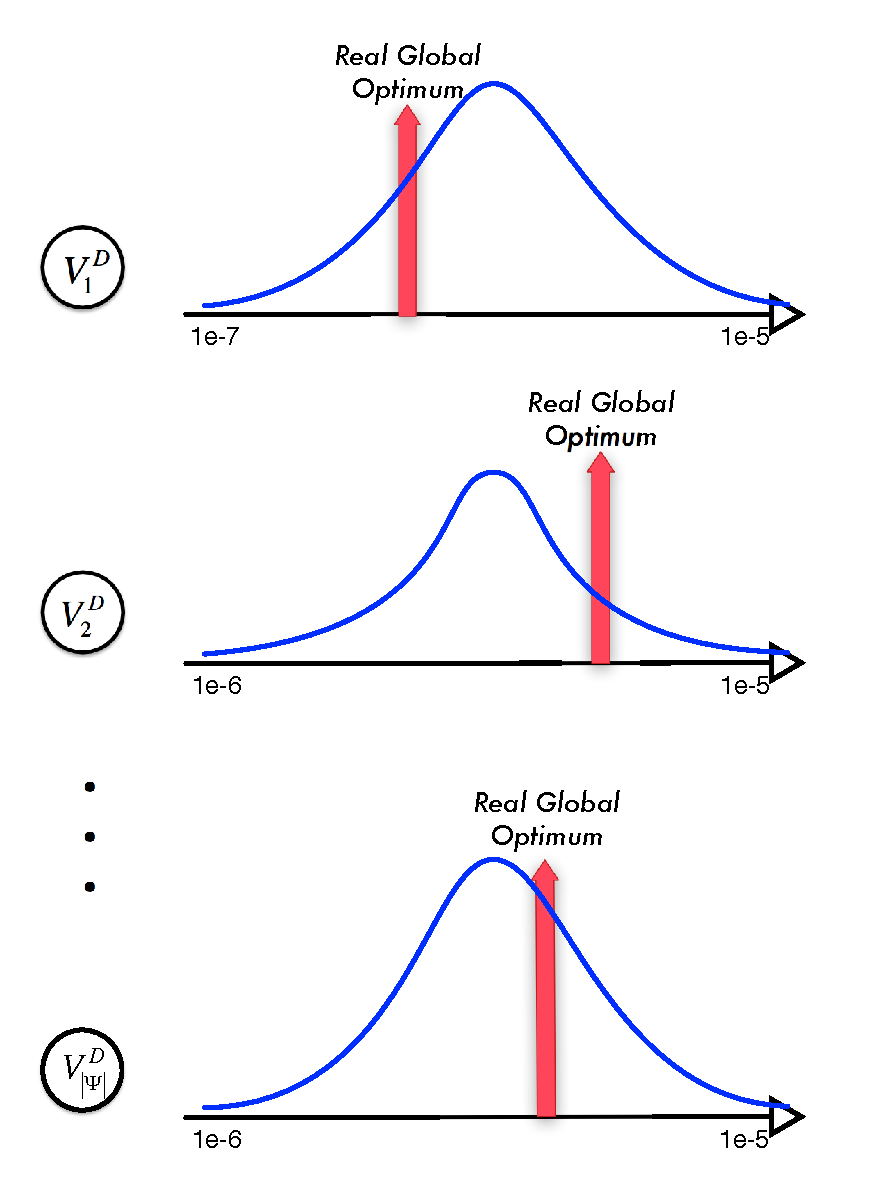
\includegraphics[width=\textwidth]{Fig/norPopDis.eps}
      \end{subfigure}
      \caption
      {
        Different distribution for stochastic simulation. (a) Population samplings for each device level variable from population and the global optimum location. (b) Normal distributions for each device level variable after normalized and the global optimum location.
      }\label{fig:optimumValleys}
  \end{figure}

  Such multi-objective simulated annealing (SA) based stochastic simulation is implemented in \cite{PerfMap_ISQED2011}. During perturbation, each swap of $V^D_m$ is referred to a uniform manufacturable range with respect to each device variable ($V^D_{M_{min}},V^D_{M_{MAX}}$). Since the range of each device variable is uncertain and continuous, the solution set can be wide. Normally, a movement among the range of $V^D_M$ is decided by the uniform probability, i.e., every movement is randomly chosen in the equal chance. As a matter of fact, some corner values are trivially unfeasible, and it is time-consuming to evaluate unfeasible solutions. Even if multi-objective SA has a good initial solution, the full range stochastic simulation accompanies with vast computing time to converge. We observe that the perturbation strategy can be performed statistically. 
    

  To ease the effort with simulation, the possibility of each movement among the range of $V^D_M$ can be manipulated. For each $V^D_M$, $N_P$ samples are collected via {\it Design Re-targeting}. Therefore, these samples construct a distribution for $V^D_M$. Since all of them are potential candidates for optimal solution, We believe that the sparser density results in less likelihood toward optimal solution. Consequently, the distribution of $V^D_M$ forecasts the performance behaviors related to probability. To extend this idea, the distribution of $V^D_M$ values can be transferred into the probability density function (PDF) and cumulative distribution function (CDF), and every movement of swap is determined by such function. Different from the uniform manufacturable range, it is closer to the behavior of performance metrics. Theoretically, the global optimum oughts to among these peaks of distributions with respect to each device variable. Roughly, performance results are quite close to real circuit simulation results such as SPICE. In other words, every prediction result from genetic based performance exploration projects to a device variable set, and the PDF-deterministic perturbation for circuit simulation benefits the convergence of multi-objective optima performance.


  \newcommand{\PFTS}{\ensuremath{\mbox{\sc ProbFineTuneSimulation}}}
  %\renewcommand{\algorithmicrequire}{\textbf{Input:}}
  %\renewcommand{\algorithmicensure}{\textbf{Output:}}
  \algloopdefx{RETURN}[1][]{\textbf{return} #1}
  \algblockdefx{FORALLP}{ENDFAP}[1]%
    {\textbf{for all }#1 \textbf{do in parallel}}%
    {\textbf{end for}}
  \begin{algorithm}[t]  
    \caption{$\PFTS(T,T_{freeze}, \Psi, r, N_s)$}\label{alg:PFTS}                       
    \begin{scriptsize}
      \begin{algorithmic}[1]
        \REQUIRE 
          \begin{tabular}{l}
            $T$: A initial temperature, $T>0$.\\
            $T_{freeze}$: Frozen temperature for annealing.\\
            $\Psi$: A set of overall device parameter values.\\
            $r$: A factor to reduce temperature T.\\
            $N_s$: Number of normal distribution sampling.\\
          \end{tabular}
        \ENSURE
          \begin{tabular}{l}
            $\hat{V^D_M}$: Optimal design parameters. \\
            $R$: Optimal performance data from simulation. \\
          \end{tabular}
        \FOR {$j = 1 \to |M|$}
          \STATE $mean_j=CalculateMean(\Psi,j)$
          \STATE $std_j=CalculateVariance(\Psi,j)$
          \STATE $pdf_{j}=normalPDFGenerator(mean_j, std_j,N_s)$
        \ENDFOR
        \FOR{$j= 1 \to |M|$}
          \STATE $V^D_{m_j} = mean_j$
        \ENDFOR
        \STATE $R=Evaluate(V^D_M),\; V^D_M = \{V^D_{m_j}| 1 \leq j \leq |M|\}$
        \WHILE {$T > T_{freeze}$}
          \FOR {$j = 1 \to |M|$}
            \STATE ${V^D_{m_j}}' = Move(pdf_j)$
          \ENDFOR
          \STATE $R'=Evaluate({V^D_M}')$
          \IF{$cost(R') \prec cost(R)$}
            \STATE $R' \gets R$
          \ELSE
            \STATE $R' \gets R\ with\ probability\ min(1,exp\{ -\frac{\delta E(cost(R'),cost(R)} {T}\})$
          \ENDIF
          \STATE $T \gets rT$
        \ENDWHILE
          \STATE $\hat{V^D_M} \gets V^D_M$
        \STATE $return\ R$          
      \end{algorithmic}
    \end{scriptsize} 
  \end{algorithm}

  As illustrated in Fig.~\ref{fig:optimumValleys} (a), while swapping according to the distribution of $V^D_M$, discrete distribution affects the accuracy of movement schedule. In addition, the original distribution is refurbished as normalized distribution. Later, the normal distribution for each device variable $V^D_M$ is obtained (shown in Fig.~\ref{fig:optimumValleys} (b)). The nearest point to the mean value from samples symbolizes higher potential to reach the global optimum. Also, the normal distribution ensures that the probability of every movement manufacturable range is feasible. On the boundary of such distribution, the probability decreases and results in less visiting while swapping. Regarding the uniform simulation, since all of samplings have equal probability, SA based simulation spends more efforts on local solution. Other than the uniform approach, this strategy forbids certain trivial simulation with worse performance.  


  In detailed implementation (shown in Algorithm~\ref{alg:PFTS}), given the variable sets, normalized distributions for each design variable are generated by calculating the mean values and standard deviations. In other words, it represents the probability density function (PDF) for that device-level variable. The Box-Muller method \cite{BoxMuller1958AMS} uses two independent random number, then it generates two standard normal distribution variables. As Eq.(\ref{eq:BoxMullerEq}) illustrated, two independent random numbers $U$ and $V$ are distributed uniformly between (0,1), then the two standard normal distribution variables $X$ and $Y$ are generated. two normal distribution variables $X'$ and $Y'$ are further obtained in terms of $\mu$ and $\sigma^2$ ($\mu$ is the mean and $\sigma^2$ is the variance). A set of PDF for each device-level variable is generated after dividing all of samplings into several intervals and calculate the number of interval sampling to get the PDF from $\Psi$. $PDF = \{ {pdf}_k | 1 \leq k \leq |M|\}$.
    

  \begin{align}{\label{eq:BoxMullerEq}}
    \begin{array}{l}
      \exists \ U\sim\mathcal{U}(0,1)\ and\ V\sim\mathcal{U}(0,1)\\
      \Rightarrow \left\{
      \begin{array}{l}
      %X=R\cos(\theta)\\
      %Y=R\sin(\theta)\\
        X=\sqrt{-2lnU}\cos(2\pi V)\\
        Y=\sqrt{-2lnU}\sin(2\pi V)\\
      \end{array}
      \right .
      X,\ Y\sim\mathcal{N}(0,1)\\
      Extend:\\
      \left\{
      \begin{array}{l}
        X'=\sqrt{-2lnU}\cos(2\pi V)\times \sigma+\mu\\
        Y'=\sqrt{-2lnU}\sin(2\pi V)\times \sigma+\mu\\
      \end{array}
      \right .
      X,\ Y\sim\mathcal{N}(\mu,\sigma^2)\\
    \end{array}
  \end{align} 

  


  We assign maximum and minimum values for each $V^D_m$ from technology design rules, and then apply {\it Probabilistic Perturbation Fine Tuning} among these variable boundaries based on multi-objective perturbation as shown in Algorithm~\ref{alg:PFTS}. The $normalPDFGenerator$ use Box-Muller method to generate PDF for each $V^D_M$ is shown in Algorithm~\ref{alg:normalPDFGenerator}.


  From Line 1 to Line 5 in Algorithm~\ref{alg:PFTS}, it illustrates the PDF generates process for each device variable $V^D_m$. Before multi-objective perturbation, the initial solution is selected. According to the PDF function for each $V^D_m$, the mean value represents a good initial point for simulation (from Lin 6 to Line 8). Thus, we obtain the the initial solution $R$ via $Evaluate(V^D_M)$ in Line 9. Later, it proposes the multi-objective SA to converge the optimal solution from Line 10 to Line 22. Originally, the $Move(pdf)$ function selects a point between $V^{D}_{m_{max}}$ to $V^{D}_{m_{min}}$ randomly. However, this kind of selection picks up the optimal value and the corner value of variable $V^D_m$ with the equal probability. To leverage the distribution of each variable $V^D_m$, we try to select next $V^D_m$ value according to different possibility. Therefore, $Move(pdf_j)$ selects value of each $V^D_m$ accord to $pdf_j$ generated by Algorithm~\ref{alg:normalPDFGenerator}. Fig.~\ref{fig:NorPDFSwap} demonstrates one example of $Move(pdf_j)$ operation. In Algorithm~\ref{alg:PFTS} Line 14, the set of device variables ${V^D_M}'$ is fed into circuit simulator to obtain result $R'$. If $R'$ dominates $R$ (or $R' \prec R$), the new solution $R'$ is accepted. The dominant relationship is defined in {\it Definition~\ref{def:Dominate}}. For the objective function in {\it Definition~\ref{def:Dominate}},we apply a composite function method to obtain the combined cost function of multi-objective values in {\it Definition~\ref{def:objective}} which is inspired by Engrand et al.~\cite{EngrandMOSA}. While $R'$ does not dominate $R$, it still has probability to accept $R$ (shown in Algorithm~\ref{alg:PFTS} Line 18) and then the temperature $T$ is cooled down factor $r$. $ProbFineTuneSimulation$ terminates when the temperature $T$ reaches $T_{freeze}$ then an optimal result $R$ is achieved.


  \newcommand{\normalPDFGenerator}{\ensuremath{\mbox{\sc normalPDFGenerator}}}
  %\renewcommand{\algorithmicrequire}{\textbf{Input:}}
  %\renewcommand{\algorithmicensure}{\textbf{Output:}}
  \algloopdefx{RETURN}[1][]{\textbf{return} #1}
  \algblockdefx{FORALLP}{ENDFAP}[1]%
  {\textbf{for all }#1 \textbf{do in parallel}}%
  {\textbf{end for}}
  \begin{algorithm}[t]  
    \caption{$\normalPDFGenerator(M, Std, N_s)$}\label{alg:normalPDFGenerator}                       
    \begin{scriptsize}
      \begin{algorithmic}[1]
        \REQUIRE 
        \begin{tabular}{l}
          $M$: Mean of population sampling.\\
          $Std$: Standard deviation of population sampling.\\
          $N_{total}$: Number of Box-Muller method sampling.\\
        \end{tabular} 
        \FOR {$j = 1 \to N_{total}$}
          \STATE $U=rand(0,1)$
          \STATE $V=rand(0,1)$
          \STATE $X=\sqrt{-2lnU}\cos(2\pi V)\times Std + M$
          \STATE $Y=\sqrt{-2lnU}\sin(2\pi V)\times Std + M$
        \ENDFOR
        \STATE $Z\gets X, Y$
        \FOR {$i = 1 \to N_s$}
          \STATE $pdf_{i}\gets \frac{NumberOfSampling(Z, i, i-1)}{N_{total}}$
        \ENDFOR
        \STATE $return\ pdf$
      \end{algorithmic}
    \end{scriptsize} 
  \end{algorithm}

  \begin{figure}[ht]
    \centering
    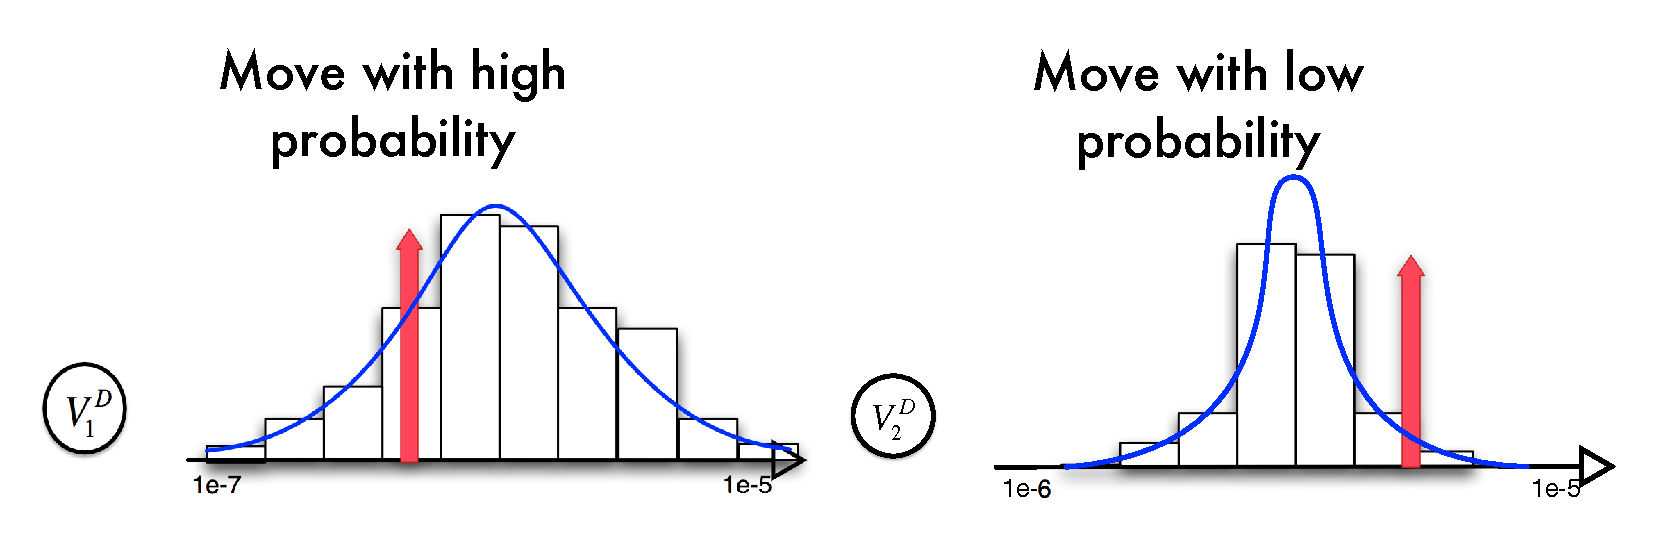
\includegraphics[width=\textwidth]{Fig/NorPDFSwap.eps}
    \caption{Swap behavior dominated by probabilistic in PDF of $V^D_m$} 
    \label{fig:NorPDFSwap}
  \end{figure}


  \newtheorem{PFTSDef}{Definition}
  %\newtheorem{Dominate}[func]{Definition}
  \begin{defi}\label{def:Dominate}
    x $\prec$ y (called x dominates y) iff $E_i(x)$ $\leq$ $E_i(y)$, for i=1,\dots ,K and $E_j(x)$ $\leq$ $E_j(y)$ for least one objective function $E_j$.
  \end{defi}

  \begin{defi}\label{def:objective}
    The composite objective function is defined, $E=\displaystyle\sum_{n=1}^{K} ln(w_if_i(x))$, where $f_1$, $\dots$ ,$f_K$ are K objectives to be optimized and $w_i$ is normalized weighting value corresponding to each objective result, for i=1, $\dots$ ,k.
  \end{defi}



  A hierarchical synthesis for circuit sizing strategy is accomplished after the optimal solution is converged when stochastic simulator or the termination requirement is met. Based on a probabilistic stochastic fine-tuning, the convergence time successfully reduced comparing to non-probabilistic approach because certain simulations of corner cases are examined via selection. 